% =====================================================================================
%  IEEE conference paper (IEEEtran) -- compile with pdfLaTeX in Overleaf.
%  Upload next to this file: fig_architecture.png, fig_login_home.png, fig_leaderboard.png,
%                            fig_copilot_audit.png, fig_blind_screening.png
%  Every number below comes from paper_results.json (12-resume pilot) or from the authors' draft
%  (100-resume benchmark, adversarial probe). Nothing is estimated.
% =====================================================================================
\documentclass[conference]{IEEEtran}

\usepackage{cite}
\usepackage{amsmath,amssymb,amsfonts}
\usepackage{graphicx}
\usepackage{textcomp}
\usepackage{xcolor}
\usepackage{booktabs}
\usepackage{array}
\usepackage{tabularx}
\usepackage{adjustbox}
\usepackage{url}
\usepackage{pgfplots}
\pgfplotsset{compat=1.16}
\graphicspath{{./}{figures/}}

\def\BibTeX{{\rm B\kern-.05em{\sc i\kern-.025em b}\kern-.08em
    T\kern-.1667em\lower.7ex\hbox{E}\kern-.125em X}}

% Verdict labels and code names
\newcommand{\verd}[1]{\textsc{#1}}
\newcommand{\flag}[1]{\texttt{\footnotesize #1}}
\newcommand{\tflag}[1]{\texttt{\scriptsize #1}}
\newcommand{\Sstrong}{\verd{Strong Hire}}
\newcommand{\Shire}{\verd{Hire}}
\newcommand{\Slean}{\verd{Lean Hire}}
\newcommand{\Sreject}{\verd{Reject}}

\begin{document}

% Previous working title (kept for reference):
% Evidence-Grounded and Bias-Aware Candidate Screening with a Deterministic Multi-Agent Council:
% Hybrid Retrieval, Skill Ontology and External Verification
\title{An Explainable Multi-Agent AI Recruitment System with Hybrid Skill Ontology, Bias-Aware Auditing, and RAG Copilot}

\author{\IEEEauthorblockN{1\textsuperscript{st} Mithila R}
\IEEEauthorblockA{\textit{Dept. of Information Science} \\
\textit{and Technology}\\
\textit{Vivekananda Institute}\\
\textit{of Technology}\\
Bengaluru, India \\
mithilaagowdaa@gmail.com}
\and
\IEEEauthorblockN{2\textsuperscript{nd} Sneha K}
\IEEEauthorblockA{\textit{Dept. of Information Science} \\
\textit{and Technology}\\
\textit{Vivekananda Institute}\\
\textit{of Technology}\\
Bengaluru, India \\
snehak2357@gmail.com}
\and
\IEEEauthorblockN{3\textsuperscript{rd} Yashaswini R}
\IEEEauthorblockA{\textit{Dept. of Information Science} \\
\textit{and Technology}\\
\textit{Vivekananda Institute}\\
\textit{of Technology}\\
Bengaluru, India \\
yashaswinirpt10@gmail.com}
}

\maketitle

% ------------------------------------------------------------------------------------
\begin{abstract}
Keyword-based applicant tracking systems (ATS) reward vocabulary rather than evidence, and recent audits show that neural resume screeners can inherit demographic bias. We present an explainable, offline-capable recruitment system that treats a skill as a claim to be evidenced. It combines a 79-skill ontology with alias normalisation and partial-credit matching, a seven-factor hybrid ranker, evidence-weighted skill coverage, data-layer blind screening, a four-agent deterministic consensus council with knock-out gates, a GitHub authenticity inspector, and a retrieval-grounded recruiter copilot behind a React interface that uses progressive disclosure. On a 12-resume pilot, the system ranks a buzzword-stuffed 0.3-year resume 10th, whereas a keyword baseline ranks it 5th and scores it identically to a genuine four-year lateral candidate (Kendall $\tau=0.667$ between the two rankings). A full screen costs 29.6~ms per resume on a laptop CPU. Scores and verdicts are invariant to name substitution ($\Delta=0.0$ over 96 runs) and stable under $\pm20\%$ weight perturbation (mean $\tau=0.969$, 200 draws). On a 100-resume synthetic benchmark the system agrees exactly with the generation labels for 46 of 100 resumes and issues no \Sstrong{} verdict, a conservative calibration that we analyse. All data are synthetic, and we state the resulting limitations explicitly.
\end{abstract}

\begin{IEEEkeywords}
resume screening, algorithmic hiring, explainable AI, fairness, multi-agent systems, retrieval-augmented generation, skill ontology
\end{IEEEkeywords}

% ====================================================================================
\section{Introduction}
Recruiters receive far more applications than they can read, and automated screening has become the first gatekeeper in many hiring pipelines. Two failure modes are well documented. First, legacy ATS products rank by lexical overlap with the job description, so a resume that lists every fashionable tool outranks one that demonstrates fewer tools with measurable results. Second, learned screeners can encode historical bias: a recruiting tool built at Amazon was reportedly abandoned after it penalised resumes associated with women~\cite{dastin}, field experiments have shown that identical resumes with different names receive different callbacks~\cite{bertrand}, and recent audits of embedding-based and generative screeners find the same pattern in modern language models~\cite{wilson,armstrong}.

Regulation is moving in the same direction. The EU Artificial Intelligence Act lists systems intended to be used for the recruitment or selection of natural persons, in particular to analyse and filter job applications and to evaluate candidates, among its high-risk applications (Annex~III, point~4(a))~\cite{euai}, which brings obligations of transparency and human oversight. A screening tool that cannot justify its ranking, expose disagreement, or hand uncertain cases to a person is therefore both ethically and legally fragile.

This paper reports the design and evaluation of a university recruitment system whose earlier version was a keyword ATS. The current system is built around one idea: \emph{a skill is a claim, and a claim needs evidence}. Our contributions are:
\begin{itemize}
\item \textbf{Evidence-weighted skill coverage.} Skills that appear only in a skills list are discounted relative to skills demonstrated in experience or project text; the discount feeds both the ranker and the final gate (Sec.~\ref{sec:math}).
\item \textbf{A seven-factor hybrid ranker} over an auditable skill ontology with partial credit, alias normalisation and fuzzy matching, with TF-IDF or dense-embedding semantics.
\item \textbf{A deterministic four-agent council} with weighted consensus, knock-out gates, individually explainable red flags, dissent reporting, a calibrated confidence value and explicit human-review triggers. A language model is optional and writes only the narrative.
\item \textbf{Defence in depth against bias:} blind screening applied before any agent sees the resume, an auditor agent that can down-weight a biased evaluator, and a counterfactual name-swap test.
\item \textbf{Adversarial temporal and structural gates} (month-aware timeline parsing, concurrent full-time employment, missing education) that a keyword or TF-IDF pipeline passes.
\item \textbf{External verification} of claimed languages through a GitHub authenticity inspector that reports uncertainty instead of guessing.
\item \textbf{A modular, offline-first implementation}: a React~19 + Vite front end with a progressive-disclosure workflow, a retrieval-grounded recruiter copilot, a Python core library and FastAPI REST services.
\end{itemize}

We organise the evaluation around five research questions. \textbf{RQ1:} does evidence-weighted screening separate genuine from keyword-stuffed candidates better than a keyword baseline? \textbf{RQ2:} are scores invariant to the candidate's name? \textbf{RQ3:} are conclusions robust to the expert-chosen weights? \textbf{RQ4:} what does a screen cost? \textbf{RQ5:} are temporal and structural anomalies that defeat a keyword or TF-IDF pipeline intercepted by explicit gates?

% ====================================================================================
\section{Related Work}
\subsection{Resume parsing and person--job fit}
Surveys of talent analytics~\cite{qin_survey} and job recommender systems~\cite{ruijt} show a shift from handcrafted features to neural models. Qin et al.\ proposed an ability-aware neural network that matches each job requirement against the candidate's experiences~\cite{qin_pjf}, and Bhatia et al.\ combined a resume parser with BERT sentence-pair classification, reporting 73\% accuracy for candidate suitability~\cite{bhatia}. Deshmukh and Dahake compared BERT and Sentence-BERT for screening and report 90\% versus 86\% accuracy, with much faster inference for the latter~\cite{deshmukh}. These systems optimise matching accuracy; they do not ask whether a matched skill is actually evidenced in the resume.

\subsection{Semantic and hybrid retrieval}
Sentence-BERT produces fixed-size sentence embeddings that can be compared by cosine similarity~\cite{sbert}, and dense retrievers outperform sparse ones on paraphrase-heavy queries while sparse methods remain strong on rare exact terms~\cite{dpr}. Okapi BM25~\cite{bm25} and TF-IDF weighting~\cite{tfidf} are the standard lexical baselines, and retrieval-augmented generation grounds language-model output in retrieved text~\cite{rag}. Our search layer fuses dense and BM25 scores at chunk level and returns evidence snippets with every hit.

\subsection{Skills, ontologies and language models}
Clavi\'e and Souli\'e show that large language models can map job-posting text to the 13{,}000-skill ESCO taxonomy through synthetic data generation and re-ranking~\cite{clavie}. Such approaches are powerful but probabilistic: a generative model can assert a skill that is not in the text. We instead use a small, auditable ontology with explicit synonym and related-skill rules.

\subsection{Bias and fairness in algorithmic hiring}
Bertrand and Mullainathan's audit study established that identical resumes with White-sounding names received substantially more callbacks than those with African-American-sounding names~\cite{bertrand}. Bogen and Rieke examined hiring algorithms across the pipeline~\cite{bogen}, and Raghavan et al.\ analysed 18 vendors of algorithmic pre-employment assessments, finding limited transparency and heavy reliance on outcome-based criteria such as the four-fifths rule~\cite{raghavan}. For language-model screeners, Wilson and Caliskan report that resumes with White-associated names were preferred in up to 85.1\% of retrieval tests~\cite{wilson}, and Armstrong et al.\ find stereotype-driven scoring in GPT-3.5~\cite{armstrong}. FA*IR gives a statistical test for fair top-$k$ rankings~\cite{fair}.

\subsection{Multi-agent deliberation and external evidence}
Multi-agent debate among language-model instances improves factuality and reasoning on benchmarks such as arithmetic (67.0\% to 81.8\%)~\cite{du}, and multi-agent referee teams yield evaluators closer to human judgement~\cite{chateval}. LLM judges also exhibit biases such as position bias~\cite{zheng}. These works study benchmark question answering and text evaluation, not hiring decisions. Hauff and Gousios matched GitHub developer profiles to job advertisements~\cite{hauff}; to our knowledge, among the works surveyed, public-repository evidence has been used to recommend developers rather than to audit the claims made on a specific resume.

\begin{table*}[t]
\caption{Representative prior work, as reported in the cited sources, and what it leaves open for this work.}
\label{tab:related}
\centering
\footnotesize
\renewcommand{\arraystretch}{1.15}
\begin{tabular}{@{}llp{5.2cm}p{5.4cm}@{}}
\toprule
Ref. & Area & Reported focus and result & Left open for this work \\
\midrule
\cite{qin_pjf}  & Person--job fit & Ability-aware neural network; interpretable attention over requirements & Skill claims not checked for evidence; no fairness stage \\
\cite{bhatia}   & Parsing + BERT  & Resume parser with BERT pair classification; 73\% suitability accuracy & No bias, evidence or uncertainty handling \\
\cite{deshmukh} & S-BERT vs BERT  & 90\% vs 86\% screening accuracy & Accuracy only; no explanation of rejections \\
\cite{clavie}   & LLM skill matching & Skill-to-ESCO matching; R-precision@10 of 61.0 (House) and 68.9 (Tech) & Probabilistic; API-dependent; no screening decision \\
\cite{wilson}   & Bias audit & Embedding retrieval: White-associated names preferred in up to 85.1\% of tests & Measures bias; does not propose a screening design \\
\cite{raghavan} & Vendor study & 18 vendors: limited transparency, outcome-based fairness & Practice review; no reference implementation \\
\cite{du}       & Multi-agent debate & Arithmetic accuracy 67.0\% $\rightarrow$ 81.8\% & Benchmarks, not gated hiring decisions \\
\bottomrule
\end{tabular}
\end{table*}

\subsection{Research gaps}
Table~\ref{tab:related} summarises representative prior work. Reading the literature against the practical requirements of a defensible screening tool, we identify the following gaps (our synthesis of the cited works, not a claim that no other work exists): (G1)~matching optimises similarity and treats a listed skill as evidence~\cite{qin_survey,ruijt,qin_pjf,bhatia,deshmukh}; (G2)~neural and LLM screeners show name and gender bias while vendor mitigation is outcome-based~\cite{wilson,armstrong,raghavan}; (G3)~regulation requires transparency and human oversight~\cite{euai} but few tools expose dissent or uncertainty; (G4)~multi-agent debate is studied for benchmarks, not gated hiring decisions~\cite{du,chateval}; (G5)~LLM skill mapping is probabilistic and API-dependent~\cite{clavie}; (G6)~repository evidence is used for matching, not for auditing resume claims~\cite{hauff}; and (G7)~generated or edited resumes can carry temporal and structural tricks (inverted dates, concurrent full-time roles, omitted education) that similarity scoring does not examine. Table~\ref{tab:gaps} maps each gap to our response.

\begin{table}[t]
\caption{Research gaps and how this work responds.}
\label{tab:gaps}
\centering
\footnotesize
\renewcommand{\arraystretch}{1.1}
\begin{tabular}{@{}lp{6.1cm}@{}}
\toprule
Gap & Response in this work \\
\midrule
G1 & Evidence-weighted coverage discounts listed-but-undemonstrated skills (Sec.~\ref{sec:math}) \\
G2 & Data-layer blind screening, auditor agent, counterfactual name-swap test \\
G3 & Verdict with red flags, dissent, confidence and human-review triggers \\
G4 & Deterministic council; LLM optional and narrative-only \\
G5 & Auditable ontology with 0.5 related-skill credit; offline fallbacks \\
G6 & GitHub inspector verifies claimed languages and reports uncertainty \\
G7 & Month-aware timeline checks and two new gates (Sec.~\ref{sec:adv}) \\
\bottomrule
\end{tabular}
\end{table}

% ====================================================================================
\section{System Architecture and Methodology}
\label{sec:arch}

\subsection{Modular architecture}
Fig.~\ref{fig:arch} shows the end-to-end pipeline. A framework-free Python core library implements every scoring algorithm. It is exposed through (i)~a FastAPI service with REST resources for jobs, resumes, screenings (including a recruiter-decision endpoint) and audits, persisted with SQLAlchemy, and (ii)~a React~19 + Vite front end. The React client extracts PDF text in the browser (pdfjs-dist) and DOCX text (mammoth) and ships a browser-side parser and scorer so that the demonstration runs fully offline; the Python core remains the reference implementation of the algorithms evaluated in Sec.~\ref{sec:exp}. The front-end data layer is organised as replaceable service modules (authentication, candidates, GitHub, mail) selected by environment variables, so that a persistent store or external APIs can be attached without changing components. In the deployed configuration the React client is served from Vercel and calls the FastAPI service on Render, which stores user accounts, sessions and the candidate pools in a MongoDB Atlas database; the relational resources keep their SQLAlchemy persistence.

\begin{figure*}[t]
\centering
\includegraphics[width=0.92\textwidth]{fig_architecture.png}
\caption{End-to-end system architecture of the explainable recruitment platform. All scoring components run locally; dense embeddings and an LLM narrative are optional.}
\label{fig:arch}
\end{figure*}

\subsection{Progressive-disclosure recruiter workflow}
The home screen is organised as three guided steps: (1)~an active-role summary, with the full competency ontology and role editor behind a disclosure control; (2)~candidate intake by upload (PDF, DOCX, TXT) or one-click benchmark pools, with a live indicator of the pool size; and (3)~a launchpad of next actions (leaderboard, comparison, interview assistant, chatbot). All controls of the earlier flat layout remain available; only their visibility is staged. The interview assistant builds a kit of 19--24 candidate-specific questions (mean 20.7 over the 162 pooled candidates) from the role family, the matched skills, the red flags and the GitHub risk of the candidate. Access is gated by a single sign-in/sign-up card; in the stand-alone configuration, account passwords are stored as per-user salted PBKDF2-HMAC-SHA256 digests~\cite{rfc8018} (200{,}000 iterations) in browser storage. In the deployed configuration authentication is delegated to the server, which hashes passwords with PBKDF2-HMAC-SHA256 (210{,}000 iterations, per-user salt), stores only the SHA-256 digest of random session tokens that expire after seven days, locks an account for 15 minutes after five wrong passwords, and verifies Google ID tokens (audience, issuer, expiry, verified e-mail, Gmail only) before it creates a session. The credential fields block copy, cut and paste but accept password-manager autofill. Fig.~\ref{fig:home} shows both screens. We did not run a usability study.

\begin{figure}[t]
\centering
\includegraphics[width=\columnwidth]{fig_login_home.png}
\caption{Progressive recruiter portal: (a)~minimalist PBKDF2 authentication card and (b)~3-step guided job vacancy and resume intake workflow.}
\label{fig:home}
\end{figure}

\subsection{Parsing and ATS quality ($S_{\mathrm{ats}}$)}
Resumes in PDF, DOCX or plain text (with an OCR fallback in the Python parser) are segmented into sections by header patterns. Employment dates are collected as month-resolution intervals. Inverted intervals ($e<s$) and future start dates are excluded from experience and reported as \flag{DATE\_INCONSISTENCY}; valid overlapping intervals are merged into a union before total experience is computed, which prevents double counting, while overlaps between non-intern full-time roles are passed to the concurrency check of Sec.~\ref{sec:math}. The ATS quality score (0--100) covers structure, contact hygiene, content density and quantified impact, and deducts up to 10 points for non-chronological or impossible date ranges. It is the seventh ranking factor, $S_{\mathrm{ats}}$.

\subsection{Skill ontology ($S_{\mathrm{tech}}$)}
The ontology contains 79 canonical skills and 353 alias entries (e.g., ``sklearn'' and ``Scikit Learn'' map to Scikit-Learn, ``k8s'' to Kubernetes). A query skill is normalised by exact alias lookup, then by punctuation-stripped lookup, then by fuzzy matching (sequence-similarity ratio above 0.88) against all aliases. Matching returns three sets: matched, partially matched and missing. Partial credit is granted only through an explicit table of 15 related pairs (e.g., FastAPI--Flask, Docker--Kubernetes) and is worth 0.5. Because every credit traces to a rule, no skill can be hallucinated. The ontology is deliberately small and auditable; its size limits coverage of specialised vocabularies, which we list as a limitation.

\subsection{Seven-factor hybrid ranking engine}
The overall score is a weighted sum of seven signals, each in $[0,100]$ (Eq.~\ref{eq:rank} and Table~\ref{tab:params}). $S_{\mathrm{tech}}$ is the partial-credit skill match percentage. $S_{\mathrm{sem}}$ is the cosine similarity between resume and job-description text, computed with 384-dimensional MiniLM embeddings (all-MiniLM-L6-v2) when the library is installed and with a scaled TF-IDF cosine~\cite{sklearn} otherwise; the backend in use is reported in the interface. $S_{\mathrm{exp}}$ compares parsed years of experience with the role's minimum: 85 plus 5 points per surplus year (capped at 100) when the minimum is met, and a proportional score (floor 25) otherwise. $S_{\mathrm{edu}}$ maps the highest parsed degree to a base score, adds a bonus for a related branch and for a high CGPA, and is capped at 100. $S_{\mathrm{proj}}$ rewards the number of projects (up to 60 points) plus up to 40 points for the share of required skills used in projects. $S_{\mathrm{cert}}$ is based on the \emph{number} of listed certifications (baseline 40 when none); credentials are counted, not validated against an issuer, which is a limitation.

\subsection{Blind screening and the Fair-Hiring Auditor}
Blind mode replaces the name by a neutral identifier, redacts e-mail, phone, location and profile links, replaces occurrences of the name in the text and neutralises gendered pronouns and honorifics, producing the only copy that the council receives (Fig.~\ref{fig:blind}). The Fair-Hiring Auditor then scores merit using only job-related evidence, reports an integrity score and bias flags, and, when it flags another agent's evidence as non-merit-based, halves that agent's consensus weight before renormalisation. Direct identifiers are removed; proxy variables such as institution prestige are \emph{flagged rather than removed}.

\begin{figure}[t]
\centering
\includegraphics[width=\columnwidth]{fig_blind_screening.png}
\caption{Fairness and bias-aware screening mode dynamically masking direct identifiers (name, contact details, location, profile links, gendered pronouns) before any agent evaluates the resume.}
\label{fig:blind}
\end{figure}

\subsection{The four-agent council}
Four agents score a candidate independently in $[0,100]$: the \emph{Tech Lead} (evidence-weighted skill coverage, architectural and craftsmanship signals, quantified impact, repository maturity and GitHub findings, including whether claimed work is in original rather than forked repositories); \emph{Culture and Retention} (tenure, progression and short stints); the \emph{Fair-Hiring Auditor} (merit-only score); and \emph{Seniority and Compensation} (level L3--L6 against the role's target, with indicative USD and INR bands). The agents then exchange rule-templated critiques; the transcript is stored and shown to the recruiter. Consensus, gates and review triggers are defined in Sec.~\ref{sec:math}.

\subsection{GitHub authenticity inspector}
The inspector extracts the handle from the resume, queries the public REST API using only the standard library, honours rate limits and caches responses. Each claimed language is marked verified, weak or unverified against repository language bytes of \emph{non-forked} repositories, because forked code is not authored work. The authenticity score combines language verification (0.55), recent activity (0.25) and repository substance (0.20). When there is nothing public to judge, the verdict is \flag{INSUFFICIENT\_PUBLIC\_DATA} with no score, because the absence of a public profile is not evidence of dishonesty.

\subsection{Retrieval-grounded recruiter copilot}
Resumes are chunked by section. A natural-language query is parsed into an experience requirement and competencies, expanded with synonyms, and scored per chunk by fusing dense and BM25 scores (Eq.~\ref{eq:fusion}). Candidate relevance combines semantic and competency-coverage scores, scaled by an experience-fit factor, and every hit carries matched and missing competencies and highlighted evidence snippets. The copilot composes its answers (headcount, skill coverage, red-flag audits, comparisons, outreach drafts) from this retrieved, scored evidence rather than from free generation; in the default configuration the response text is template-based and needs no language model (Fig.~\ref{fig:copilot}). The web client's copilot additionally keeps the conversation context (pronouns, ordinal references to the last list, ``show more''), asks which candidate is meant when two candidates share a name, and offers follow-up suggestions; it still answers only from the loaded pool. All components degrade without network access: MiniLM falls back to TF-IDF, the LLM narrative to rule-based text, and the GitHub widget offers a clearly labelled simulated mode for demonstrations.

\begin{figure}[t]
\centering
\includegraphics[width=\columnwidth]{fig_copilot_audit.png}
\caption{Natural-language talent copilot with red-flag audit forensics and personalised, evidence-based outreach drafting.}
\label{fig:copilot}
\end{figure}

% ====================================================================================
\section{Mathematical Formulation and Multi-Agent Scoring}
\label{sec:math}

\subsection{Problem statement}
Given a resume $x$ with claimed skills $S(x)$ and evidence $E(x)\subseteq S(x)$, and a job description $J$ with required skills $R$, the system must output a score, a categorical verdict and an explanation such that: (i)~the output is invariant to protected attributes inferred from the name or contact details; (ii)~claims in $S(x)\setminus E(x)$ are discounted; (iii)~every verdict is accompanied by the features, rules and disagreements that produced it; (iv)~uncertain cases are flagged for human review; and (v)~the pipeline runs without network access.

\subsection{Hybrid ranking score}
The final score is
\begin{multline}
S = 0.35\,S_{\mathrm{tech}} + 0.20\,S_{\mathrm{sem}} + 0.15\,S_{\mathrm{exp}} \\
 + 0.10\,S_{\mathrm{edu}} + 0.10\,S_{\mathrm{proj}} + 0.05\,S_{\mathrm{cert}} + 0.05\,S_{\mathrm{ats}},
\label{eq:rank}
\end{multline}
with weights renormalised if a user supplies custom weights ($S=\sum_i w_i s_i / \sum_i w_i$).

\subsection{Evidence-weighted skill coverage}
Let $L\subseteq R$ be the required skills found anywhere in the resume and $E\subseteq L$ those that also occur outside the skills block (experience, projects). The block is stripped by detecting its header and ending it at the next section header. Evidence-weighted coverage is
\begin{equation}
c_{\mathrm{ev}} = \frac{|E| + 0.5\,(|L|-|E|)}{|R|},
\label{eq:cev}
\end{equation}
so a skill that is claimed but never demonstrated earns half credit. The ratio $(|L|-|E|)/|L|$ of unevidenced listed skills drives the \flag{UNVERIFIED\_SKILL\_CLAIMS} flag.

\subsection{Council consensus, verdicts and gates}
With agent scores $a_{\mathrm{tech}}, a_{\mathrm{merit}}, a_{\mathrm{culture}}, a_{\mathrm{level}}$, the consensus is
\begin{equation}
C = 0.35\,a_{\mathrm{tech}} + 0.25\,a_{\mathrm{merit}} + 0.20\,a_{\mathrm{culture}} + 0.20\,a_{\mathrm{level}},
\label{eq:consensus}
\end{equation}
mapped to \Sstrong{} ($C\ge80$), \Shire{} ($\ge68$), \Slean{} ($\ge55$) or \Sreject{}. Gates override the average so that a high mean cannot hide a fatal flaw: $c_{\mathrm{ev}}<0.25$ forces \Sreject{}; $c_{\mathrm{ev}}<0.5$ caps the verdict at \Slean{}; two high-severity red flags force \Sreject{}; one caps at \Slean{}. Nine red-flag codes carry a severity and a detail string: \flag{EXPERIENCE\_DEFICIT}, \flag{REQUIRED\_SKILLS\_MISSING}, \flag{UNVERIFIED\_SKILL\_CLAIMS}, \flag{SKILL\_STUFFING}, \flag{NO\_QUANTIFIED\_IMPACT}, \flag{LEVEL\_MISMATCH}, \flag{DATE\_INCONSISTENCY}, \flag{CONCURRENT\_EMPLOYMENT\_CONFLICT} and \flag{MISSING\_EDUCATION}.

\subsection{Temporal and structural gates}
\label{sec:gates}
Let $m(y,\mathrm{mon})=12y+\mathrm{mon}$ be a month index and $t_0$ the current month. A role with interval $[s,e]$ is date-inconsistent (high severity) if $e<s$ or $s>t_0$. For two non-intern full-time roles $i,j$ the overlap is
\begin{equation}
o_{ij}=\max\bigl(0,\;\min(e_i,e_j)-\max(s_i,s_j)\bigr)\ \text{months},
\end{equation}
and \flag{CONCURRENT\_EMPLOYMENT\_CONFLICT} (high severity) is raised when
\begin{equation}
o_{ij}\ge 6\;\wedge\;\mathrm{loc}(i)\not\sim \mathrm{loc}(j),
\label{eq:concurrent}
\end{equation}
where $\mathrm{loc}(i)\not\sim\mathrm{loc}(j)$ means that the two on-site locations are in different countries and neither role is marked remote. \flag{MISSING\_EDUCATION} (medium severity) is raised when no academic credential is parsed; it subtracts 10 points of confidence and caps \Sstrong{} at \Shire{}.

\subsection{Confidence, dissent and human review}
Confidence is $100-1.2\sigma$ minus penalties for a missing timeline, no parsed skills or very short text, where $\sigma$ is the standard deviation of the agent scores. An agent whose score deviates from $C$ by more than 20 points is reported as dissent. A human review is requested when a bias flag is high, integrity is below 70, confidence is below 55, or $C$ lies within 2 points of a verdict boundary. The council is thus a decision-support device, not an autonomous decision-maker.

\subsection{Rank agreement and sensitivity}
Rank agreement between two rankings is measured by Kendall's $\tau$~\cite{kendall}. For the weight-sensitivity study each ranker weight $w_i$ is replaced by $\tilde w_i=w_i u_i/\sum_k w_k u_k$ with $u_i\sim\mathcal U[0.8,1.2]$, and each council weight likewise. Name invariance is measured by
\begin{equation}
\Delta_{\mathrm{score}}=\max_{n\in\mathcal N}\bigl|S(x_n)-S(x)\bigr|,
\end{equation}
where $x_n$ is $x$ with the name replaced by $n\in\mathcal N$ in both the name field and the text.

\subsection{Search fusion}
The chunk score of a query $q$ is
\begin{equation}
\mathrm{score}(q,d)=\alpha\,\mathrm{dense}(q,d)+(1-\alpha)\,\mathrm{BM25}(q,d),\quad \alpha=0.55,
\label{eq:fusion}
\end{equation}
with BM25 parameters $k_1=1.5$, $b=0.75$.

\begin{table}[t]
\caption{Decision-logic parameters (all configurable; none learned).}
\label{tab:params}
\centering
\footnotesize
\renewcommand{\arraystretch}{1.1}
\begin{tabular}{@{}lp{5.6cm}@{}}
\toprule
Component & Value \\
\midrule
Ranker weights & tech .35, semantic .20, experience .15, education .10, projects .10, certifications .05, ATS quality .05 \\
Skill credit & matched 1.0, related 0.5 (15 pairs), missing 0 \\
Ontology & 79 canonical skills, 353 aliases, fuzzy ratio $>0.88$ \\
Council weights & tech .35, merit .25, culture .20, level .20 \\
Verdict thresholds & \Sstrong{} $\ge80$, \Shire{} $\ge68$, \Slean{} $\ge55$ \\
Coverage gates & $c_{\mathrm{ev}}<0.25\rightarrow$ \Sreject{}; $<0.5\rightarrow$ cap \Slean{} \\
Flag gates & $\ge2$ high flags $\rightarrow$ \Sreject{}; 1 high $\rightarrow$ cap \Slean{} \\
Adversarial gates & $e<s$ or $s>t_0$ (high); $o_{ij}\ge6$ months, different countries (high); no education: $-10$ confidence, cap \Shire{} \\
Review triggers & bias flag; integrity $<70$; confidence $<55$; $|C-\text{threshold}|\le2$ \\
Role families & eight (ML, DevOps/SRE, full-stack AI, data platform, backend, AI safety, BI, Python/FastAPI) \\
Search fusion & $\alpha=0.55$ dense; BM25 $k_1=1.5$, $b=0.75$ \\
\bottomrule
\end{tabular}
\end{table}

% ====================================================================================
\section{Experimental Setup and Datasets}
\label{sec:exp}
The evaluation has three parts. \textbf{Pilot study (12 resumes, one job).} Eight synthetic resumes shipped with the project (an ML engineer, a full-stack developer, a cloud/DevOps engineer, a backend developer, a data analyst, a fresher, a deliberately flawed buzzword resume and a resume with missing sections) plus four purpose-written test cases that probe specific behaviours: TC1 (strong candidate), TC2 (buzzword-stuffed), TC3 (lateral partial match) and TC4 (corrupt format). The job is Machine Learning Engineer with 17 required skills and a 2-year minimum. \textbf{Benchmark study (100 resumes).} Synthetic resumes over eight role families, generated with language-model assistance from role-specific specifications (required stack, tenure, production metrics, GitHub handle) under four archetypes with fixed proportions: 20 strong hires, 45 lean hires, 25 buzzword exaggerators (35 or more stuffed skills, no metrics, forked tutorial repositories) and 10 chronology or formatting anomalies; the last two form the 35 reject profiles. \textbf{Adversarial probe.} The first 20 benchmark resumes (ten ML, ten DevOps/SRE) plus targeted anomalies were run through the pre-upgrade and upgraded pipelines.

\textbf{Interface demonstration pool.} The React interface additionally ships a 50-candidate pool, shown in Fig.~\ref{fig:leader}, for demonstration. It was not used for any quantitative claim in this paper.

\textbf{Mode and baseline.} Offline TF-IDF semantics (MiniLM not installed) and no LLM; Python 3.11.9 on a Windows laptop CPU, sequential, single process. The baseline is a keyword-matching score modelled on the earlier ATS: the percentage of required skills whose name appears anywhere in the resume text. \textbf{Metrics.} Kendall's $\tau$; verdict agreement with generation labels; name-swap $\Delta_{\mathrm{score}}$; Precision@3 and Recall@3 for retrieval; and per-stage latency. \textbf{Reproducibility.} The verification harness and the experiment script regenerate every number for the pilot; the sensitivity study uses a fixed random seed; the benchmark generator, manifest and run logs accompany the repository [link to be added before submission].

% ====================================================================================
\section{Results and Discussion}

\subsection{Processing latency (RQ4)}
Table~\ref{tab:latency} reports per-stage cost on the 12-resume pool. A full screen takes 29.58~ms per candidate, i.e.\ about 33.8 candidates per second on a single CPU thread. Parsing dominates (61\%); hybrid ranking is the cheapest stage. Absolute timings depend on hardware and exclude dense-embedding inference, which was not installed, and the browser rendering cost of the React client. Cost is linear in the number of resumes $N$: parsing and the council are $O(1)$ per resume, ranking adds a TF-IDF fit over the pool, and search builds a chunk index once and caches it by content fingerprint.

\begin{table}[t]
\caption{Per-resume processing latency (12-resume pool, TF-IDF backend, single thread).}
\label{tab:latency}
\centering
\footnotesize
\begin{tabular}{@{}lrr@{}}
\toprule
Stage & Latency (ms) & Share \\
\midrule
Resume parsing & 18.01 & 60.9\% \\
Hybrid scoring and ranking & 3.78 & 12.8\% \\
Multi-agent consensus & 7.79 & 26.3\% \\
\midrule
\textbf{End-to-end} & \textbf{29.58} & 100\% \\
\bottomrule
\end{tabular}
\end{table}

\subsection{Ranking divergence from the keyword baseline (RQ1)}
Table~\ref{tab:pilot} lists the 12 pilot results. The two rankings agree on the extremes (Kendall $\tau=0.667$) but diverge where the design intends (Fig.~\ref{fig:bars}). The keyword baseline scores TC2, a resume with 0.3 years of experience, one quantified result and a long list of fashionable tools, at 47.1\%, identical to TC3, a four-year backend engineer, and ranks it 5th; the second buzzword resume (Mehta) is ranked 3rd. The proposed ranker places them 10th and 6th, and separates TC2 from TC3 by 19.7 points (41.6 versus 61.3). A value of $\tau=0.667$ indicates substantial disagreement between the rankings; it does not by itself show \emph{which} ranking is correct. The evidence for correctness here is the case analysis: the demotion of the two buzzword resumes is explained by the evidence mechanism below, but with one pool of 12 synthetic resumes we claim a mechanism, not a statistical effect.

\begin{table*}[t]
\caption{Results on the 12-resume pilot pool (baseline = keyword match \%, proposed = hybrid score \%, rank in parentheses, council = consensus $C$). $\dagger$: parsed years for TC4 reflect its inconsistent dates.}
\label{tab:pilot}
\centering
\footnotesize
\renewcommand{\arraystretch}{1.1}
\begin{tabular}{@{}rlrccrl@{}}
\toprule
\# & Resume & Years & Baseline (rank) & Proposed (rank) & Council $C$ & Council verdict \\
\midrule
1  & TC1 Gold standard           & 3.0 & 100.0 (1)  & 88.1 (1)  & 91.4 & \Sstrong \\
2  & Rahul Nair (ML)             & 2.5 & 88.2 (2)   & 82.3 (2)  & 83.2 & \Sstrong \\
3  & TC3 Lateral match           & 4.0 & 47.1 (4)   & 61.3 (3)  & 76.0 & \Slean \\
4  & Sneha Kulkarni (full-stack) & 5.0 & 41.2 (6)   & 56.0 (4)  & 66.2 & \Slean \\
5  & Vikram Singh (DevOps)       & 4.0 & 29.4 (9)   & 50.1 (5)  & 61.5 & \Sreject \\
6  & Kavita Mehta (buzzwords)    & 1.0 & 52.9 (3)   & 47.4 (6)  & 48.1 & \Sreject \\
7  & Aarav Sharma (backend)      & 1.5 & 35.3 (7)   & 46.1 (7)  & 66.2 & \Slean \\
8  & Ananya Roy (fresher)        & 0.5 & 35.3 (8)   & 46.1 (8)  & 44.1 & \Sreject \\
9  & Priya Patel (analyst)       & 2.0 & 23.5 (10)  & 45.3 (9)  & 57.4 & \Sreject \\
10 & TC2 Buzzword fail           & 0.3 & 47.1 (5)   & 41.6 (10) & 50.3 & \Sreject \\
11 & TC4 Corrupt format          & 9.0$^\dagger$ & 0.0 (12) & 34.0 (11) & 38.5 & \Sreject (human review) \\
12 & Edge: missing sections      & 0.0 & 5.9 (11)   & 28.3 (12) & 27.4 & \Sreject (human review) \\
\bottomrule
\end{tabular}
\end{table*}

\begin{figure}[t]
\centering
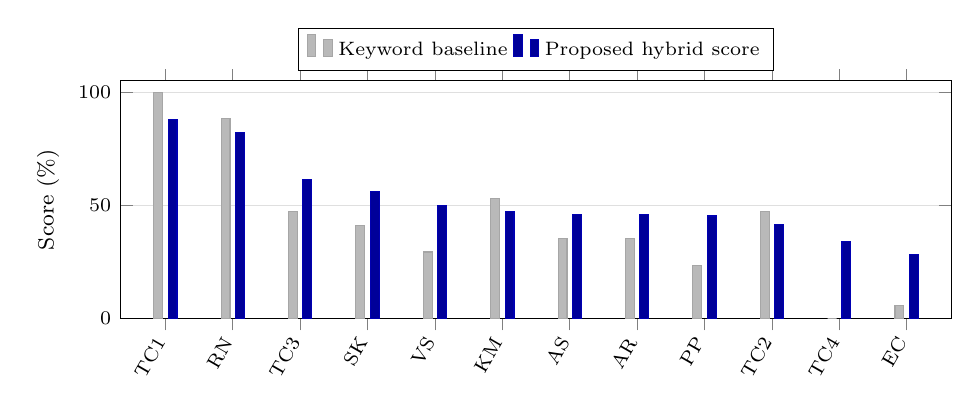
\begin{tikzpicture}
\begin{axis}[
  ybar, bar width=3.2pt, width=\columnwidth, height=4.6cm,
  symbolic x coords={TC1,RN,TC3,SK,VS,KM,AS,AR,PP,TC2,TC4,EC},
  xtick=data, x tick label style={rotate=60,anchor=east,font=\scriptsize},
  ymin=0, ymax=105, ylabel={Score (\%)}, ylabel style={font=\footnotesize},
  tick label style={font=\scriptsize},
  legend style={at={(0.5,1.04)},anchor=south,legend columns=2,font=\scriptsize},
  enlarge x limits=0.06, ymajorgrids, grid style={gray!25}]
\addplot[fill=gray!55,draw=gray!70] coordinates {(TC1,100.0)(RN,88.2)(TC3,47.1)(SK,41.2)(VS,29.4)(KM,52.9)(AS,35.3)(AR,35.3)(PP,23.5)(TC2,47.1)(TC4,0.0)(EC,5.9)};
\addplot[fill=blue!60!black,draw=blue!70!black] coordinates {(TC1,88.1)(RN,82.3)(TC3,61.3)(SK,56.0)(VS,50.1)(KM,47.4)(AS,46.1)(AR,46.1)(PP,45.3)(TC2,41.6)(TC4,34.0)(EC,28.3)};
\legend{Keyword baseline, Proposed hybrid score}
\end{axis}
\end{tikzpicture}
\caption{Keyword baseline versus proposed score for the 12 pilot resumes (abbreviations as in Table~\ref{tab:pilot}; KM and TC2 are the buzzword resumes that the baseline over-ranks).}
\label{fig:bars}
\end{figure}

\subsubsection{Evidence mechanism}
Table~\ref{tab:evidence} shows why. TC2 lists 8 required skills but evidences only 1 (unevidenced ratio 0.90), giving $c_{\mathrm{ev}}=0.27$ (TC3: 0.47; TC1: 0.97). Its council consensus of 50.3 falls below the 55-point \Slean{} threshold, and the resulting \Sreject{} carries the flags \flag{EXPERIENCE\_DEFICIT}, \flag{UNVERIFIED\_SKILL\_CLAIMS} and \flag{SKILL\_STUFFING}. TC3 keeps \Slean{}: FastAPI is credited at 0.5 through Flask, while PyTorch and the deep-learning stack are reported missing, which is what a recruiter should hear about a lateral candidate. TC4 illustrates uncertainty handling: with no parsed skills and inverted dates the ATS quality score is 23/100, confidence falls to 32.8 and the council requests human review instead of issuing a confident verdict.

\begin{table}[t]
\caption{Council evidence metrics and flags for the four test cases. $\dagger$: human review requested.}
\label{tab:evidence}
\centering
\footnotesize
\renewcommand{\arraystretch}{1.15}
\begin{adjustbox}{max width=\columnwidth}
\begin{tabular}{@{}lcccll@{}}
\toprule
Case & Listed/evid. & $c_{\mathrm{ev}}$ & Quant. & Verdict & Red flags \\
\midrule
TC1 & 17/16 & 0.97 & 9 & \Sstrong & none \\
TC2 & 8/1   & 0.27 & 1 & \Sreject & \shortstack[l]{\tflag{EXP\_DEFICIT},\\\tflag{UNVERIFIED},\\\tflag{STUFFING}} \\
TC3 & 8/8   & 0.47 & 5 & \Slean   & \shortstack[l]{\tflag{REQ\_SKILLS}\\\tflag{\_MISSING}} \\
TC4 & 0/0   & 0.00 & 0 & \Sreject$^{\dagger}$ & \shortstack[l]{\tflag{DATE\_INCONS.},\\\tflag{NO\_IMPACT}} \\
\bottomrule
\end{tabular}
\end{adjustbox}
\end{table}

\subsection{Ablation of evidence weighting and gates}
We re-ran the council with evidence weighting disabled (coverage from listed skills only, no unevidenced-skill penalty) and, separately, with the red-flag gates disabled (Table~\ref{tab:ablation}). Without evidence weighting, every consensus score rises by 0.7--4.9 points; TC2 rises from 50.3 (\Sreject) to 55.2 and is promoted to \Slean{}, just above the 55-point boundary, and Vikram Singh, a cloud/DevOps resume that lists several required ML skills, is promoted likewise; the other ten verdicts are unchanged. The second change is a reminder that evidence weighting is a deliberate trade-off: it penalises resumes whose skills appear only in lists, which can hurt terse but honest resumes, and is why such cases are routed to human review rather than hidden. Disabling the red-flag gates changed no verdict on this pool, because the flagged candidates already fall below the threshold; the gates are a safety net that this small pool does not exercise, and we claim no empirical benefit for them here (the adversarial probe of Sec.~\ref{sec:adv} is where they matter).

\begin{table}[t]
\caption{Ablation on the 12-resume pool: council consensus $C$ with and without evidence weighting. Verdict changes are in bold.}
\label{tab:ablation}
\centering
\footnotesize
\renewcommand{\arraystretch}{1.1}
\begin{adjustbox}{max width=\columnwidth}
\begin{tabular}{@{}lcccl@{}}
\toprule
Resume & Full & No evid. & $\Delta C$ & Verdict change \\
\midrule
TC1 Gold standard & 91.4 & 92.1 & +0.7 & -- \\
Rahul Nair        & 83.2 & 84.6 & +1.4 & -- \\
Aarav Sharma      & 66.2 & 66.9 & +0.7 & -- \\
Vikram Singh      & 61.5 & 62.9 & +1.4 & \textbf{\Sreject$\rightarrow$\Slean} \\
Priya Patel       & 57.4 & 58.8 & +1.4 & -- \\
TC2 Buzzword fail & 50.3 & 55.2 & +4.9 & \textbf{\Sreject$\rightarrow$\Slean} \\
Kavita Mehta      & 48.1 & 50.3 & +2.2 & -- \\
Ananya Roy        & 44.1 & 44.8 & +0.7 & -- \\
Edge: missing sections & 27.4 & 28.1 & +0.7 & -- \\
\midrule
\multicolumn{5}{@{}l}{Red-flag gates disabled: 0 verdict changes (12 resumes).} \\
\bottomrule
\end{tabular}
\end{adjustbox}
\end{table}

\subsection{Demographic robustness: counterfactual name swap (RQ2)}
Following the audit design of~\cite{bertrand}, each of the 12 resumes was re-scored with four names used in that study (Emily Walsh, Greg Baker, Lakisha Washington, Jamal Jackson) substituted in both the name field and the text, with and without blind mode: $12\times4\times2=96$ runs. In all runs the hybrid score and the council consensus were identical to the unmodified resume (Table~\ref{tab:nameswap}). This is expected for a deterministic pipeline in which the name is never a scoring feature, so \emph{the invariance holds in standard mode as well as in blind mode}. It should not be over-read: it demonstrates invariance for the TF-IDF backend and the rule-based council, not for dense embeddings or an LLM narrative, which are exactly the components where~\cite{wilson,armstrong} observe bias. Blind mode is therefore defence in depth: it enforces invariance at the data layer for those optional components and for the interface, and testing it with MiniLM and an LLM is future work.

\begin{table}[t]
\caption{Name-swap experiment: maximum score change over all substitutions ($\Delta_{\mathrm{score}}$, points).}
\label{tab:nameswap}
\centering
\footnotesize
\begin{tabular}{@{}lccc@{}}
\toprule
Mode & Hybrid score $\Delta$ & Council $\Delta$ & Runs \\
\midrule
Standard & 0.00 & 0.00 & 48 \\
Blind    & 0.00 & 0.00 & 48 \\
\bottomrule
\end{tabular}
\end{table}

\subsection{Sensitivity to the heuristic weights (RQ3)}
Because the weights are expert-chosen, we perturbed each ranker weight by a random factor in $[0.8,1.2]$ (renormalised, 200 Monte Carlo draws) and each council weight likewise (50 draws $\times$ 12 resumes). Table~\ref{tab:sens} shows that rankings remained close to the default (mean $\tau=0.969$, minimum $0.879$); the top-1 candidate and the top-3 set were unchanged in all 200 draws, and the council verdict of every resume was unchanged in all 600 evaluations. The conclusions of the ranking analysis therefore do not hinge on exact weight values within this $\pm20\%$ range, although larger changes and learned weights remain untested.

\begin{table}[t]
\caption{Monte Carlo weight-perturbation analysis ($\pm20\%$).}
\label{tab:sens}
\centering
\footnotesize
\begin{tabular}{@{}lr@{}}
\toprule
Quantity & Value \\
\midrule
Ranker draws & 200 \\
Mean Kendall $\tau$ vs.\ default & 0.969 \\
Minimum Kendall $\tau$ & 0.879 \\
Top-1 candidate stability & 100.0\% \\
Top-3 set stability & 100.0\% \\
Council verdict stability (600 evaluations) & 100.0\% \\
\bottomrule
\end{tabular}
\end{table}

\subsection{Talent-search retrieval quality}
We issued eight natural-language queries (e.g., ``Engineers with 3+ years of Python and Git'') and took as relevant the resumes whose parsed skills contain every queried skill and whose experience meets the stated minimum. BM25 only, dense (TF-IDF fallback) only and the hybrid fusion at $\alpha=0.55$ all obtained Precision@3 of 91.7\% and Recall@3 of 100.0\% (Table~\ref{tab:retrieval}). On a 12-resume pool the task is saturated, so this test confirms the correctness of the search but \emph{cannot show an advantage for fusion}; evaluating dense and hybrid retrieval with MiniLM on a larger pool with paraphrased queries is future work, and we make no superiority claim.

\begin{table}[t]
\caption{Retrieval quality (8 queries, 12 resumes).}
\label{tab:retrieval}
\centering
\footnotesize
\begin{tabular}{@{}lcc@{}}
\toprule
Retriever & Precision@3 & Recall@3 \\
\midrule
BM25 only                         & 91.7\% & 100.0\% \\
Dense only (TF-IDF fallback)      & 91.7\% & 100.0\% \\
Hybrid, $\alpha=0.55$             & 91.7\% & 100.0\% \\
\bottomrule
\end{tabular}
\end{table}

\subsection{Scaled 100-resume multi-role benchmark}
Table~\ref{tab:bench} reports the verdict distribution per role (94 of 100 resumes carry at least one red flag; the most frequent flags were \flag{REQUIRED\_SKILLS\_MISSING} (70), \flag{NO\_QUANTIFIED\_IMPACT} (67), \flag{EXPERIENCE\_DEFICIT} (40) and \flag{LEVEL\_MISMATCH} (12)). Exact agreement is defined strictly: a strong-hire profile should receive \Sstrong{}, a lean-hire profile \Shire{} or \Slean{}, and a reject profile \Sreject{}. Table~\ref{tab:confusion} gives the confusion matrix: exact agreement is 46 of 100 (46.0\%). The gross errors that matter most for a decision-support tool did not occur: no strong-hire profile was rejected and no reject profile received \Sstrong{}. The results also expose weaknesses that we do not hide. The system never issued \Sstrong{} on this benchmark (strong-hire recall 0 of 20), which we attribute to the seniority agent's level gate, since senior-level (L5) experience was not fully evidenced in the resume text; the mean consensus of the reject profiles (62.0) is slightly higher than that of the lean-hire profiles (60.1), so the score alone does not order these groups; and reject recall is only 11 of 35. Agreement with labels that the generator itself assigned measures consistency with the specification, not hiring accuracy, and we report no accuracy figure beyond the confusion matrix.

\begin{table}[t]
\caption{100-resume benchmark by role. Labels (by construction) and verdicts are given as Strong / Lean-or-Hire / Reject.}
\label{tab:bench}
\centering
\footnotesize
\renewcommand{\arraystretch}{1.05}
\begin{tabular}{@{}lcccc@{}}
\toprule
Role & $n$ & Labels (S/L/R) & Verdicts (S/L/R) & Flagged \\
\midrule
Senior ML engineer        & 13  & 3/6/4   & 0/11/2 & 10 \\
Cloud DevOps and SRE lead & 13  & 3/5/5   & 0/11/2 & 13 \\
Full-stack AI engineer    & 13  & 3/5/5   & 0/12/1 & 10 \\
Data platform engineer    & 13  & 3/5/5   & 0/13/0 & 13 \\
Backend systems architect & 12  & 2/6/4   & 0/11/1 & 12 \\
AI safety and alignment   & 12  & 2/6/4   & 0/4/8  & 12 \\
BI and analytics lead     & 12  & 2/6/4   & 0/6/6  & 12 \\
Python/FastAPI developer  & 12  & 2/6/4   & 0/11/1 & 12 \\
\midrule
\textbf{All roles}        & \textbf{100} & \textbf{20/45/35} & \textbf{0/79/21} & \textbf{94} \\
\bottomrule
\end{tabular}
\end{table}

\begin{table}[t]
\caption{Confusion matrix: generation label (rows) versus system verdict (columns: \Sstrong, \Shire{} or \Slean, \Sreject).}
\label{tab:confusion}
\centering
\footnotesize
\begin{adjustbox}{max width=\columnwidth}
\begin{tabular}{@{}lccc|c@{}}
\toprule
Label & Strong & Hire/Lean & Reject & Mean $C$ \\
\midrule
Strong (20) & 0 & 20 & 0  & 71.2 \\
Lean (45)   & 0 & 35 & 10 & 60.1 \\
Reject (35) & 0 & 24 & 11 & 62.0 \\
\bottomrule
\end{tabular}
\end{adjustbox}
\end{table}

\subsection{Adversarial edge-case stress testing (RQ5)}
\label{sec:adv}
The first 20 benchmark resumes were run through the pre-upgrade pipeline (TF-IDF backend, rule-based council, no temporal gates). The four strong profiles all received \Sstrong{} and all five buzzword profiles were rejected with \flag{EXPERIENCE\_DEFICIT} and \flag{UNVERIFIED\_SKILL\_CLAIMS}. The anomaly probes, however, were not caught (Table~\ref{tab:adv}). Candidate~019 lists a senior role as ``Jul 2026--Jan 2024''; the old parser discarded the inverted interval, so the resume was scored on a 2.0-year history and still received \Shire{} (72.5). Candidate~013 lists a full-time on-site role in San Jose from March 2023 concurrent with a full-time role in Bengaluru from January 2022 to August 2025, an overlap of 29 months; it received \Sstrong{} (89.7) with no red flag. Two further probes show the same blind spots (C1, C2). Under the upgraded pipeline the gates of Sec.~\ref{sec:gates} cap 019, 013 and C1 at \Slean{}, and C2 drops from \Sstrong{} to \Shire{}; the consensus of 013 (89.0) would otherwise map to \Sstrong{}.

This probe is a \emph{regression case study}, not a held-out detection rate: the gates were written after these failures were observed, so catching the same four resumes shows that the fix works, not that the gates generalise to unseen fraud patterns. The ``before'' values were measured on the pre-upgrade pipeline and the ``after'' values on the upgraded one, whose parser and scoring also changed, so the score differences are not attributable to the gates alone; the verdict caps are. The exercise also shows why the semantic component cannot see these attacks: an inverted date range or a second employer is invisible to TF-IDF and embedding similarity, and only an explicit timeline model exposes them.

\begin{table}[t]
\caption{Adversarial probes: verdicts before and after the new gates (consensus score in parentheses).}
\label{tab:adv}
\centering
\footnotesize
\renewcommand{\arraystretch}{1.2}
\begin{adjustbox}{max width=\columnwidth}
\begin{tabular}{@{}lp{1.9cm}llp{2.2cm}@{}}
\toprule
ID & Defect & Before & After & Flag \\
\midrule
019 & Inverted dates, Jul 2026--Jan 2024 & \shortstack[l]{\Shire\\(72.5)} & \shortstack[l]{\Slean\\(73.5)} & \tflag{DATE\_INCON.} \\
013 & Concurrent full-time, San Jose and Bengaluru & \shortstack[l]{\Sstrong\\(89.7)} & \shortstack[l]{\Slean\\(89.0)} & \tflag{CONCURRENT\_EMPL.} \\
C1  & Inverted dates, strong profile & \shortstack[l]{\Shire\\(78.6)} & \shortstack[l]{\Slean\\(73.2)} & \tflag{DATE\_INCON.} \\
C2  & No education, no phone or LinkedIn & \shortstack[l]{\Sstrong\\(92.6)} & \shortstack[l]{\Shire\\(78.6)} & \tflag{MISSING\_EDU.} \\
\bottomrule
\end{tabular}
\end{adjustbox}
\end{table}

\subsection{Recruiter interface for human review}
The interface makes these outputs directly usable. The screening leaderboard (Fig.~\ref{fig:leader}) shows the candidate count, the active model backend and the active role, a hybrid-retrieval search bar with prompt shortcuts, and ranked candidate cards (or a compact table) with score bars, evidence excerpts, matched skills, red-flag counts and the council verdict, filterable by verdict. The candidate deep-dive shows the four council scorecards, the predicted level and indicative compensation band, and a replayable cross-examination debate. Blind mode masks identities throughout. We did not run a usability study; whether these views help recruiters decide better or faster is future work.

\begin{figure}[t]
\centering
\includegraphics[width=\columnwidth]{fig_leaderboard.png}
\caption{Executive screening leaderboard showing candidate ranking, run telemetry and the seven-factor match breakdown, with the 50-candidate demonstration pool loaded (interface demonstration only; not an evaluation set).}
\label{fig:leader}
\end{figure}

\subsection{Limitations and threats to validity}
\textbf{Circularity.} Every resume is synthetic, was authored with knowledge of the system's rules, and carries a label that the generator itself assigned, so agreement with those labels shows consistency with the specification, not accuracy on real hiring outcomes. The temporal gates were designed in response to failures observed on the benchmark's own anomaly cases. Deployment on uncurated applicant pools with recruiter judgements as ground truth is the decisive test. \textbf{Calibration.} The council was conservative at the top and permissive at the bottom of the scale (0 of 20 strong profiles promoted; 11 of 35 reject profiles rejected); recalibration against recruiter decisions is required before verdict categories are used operationally. \textbf{Heuristic parameters.} Weights, thresholds and gates are expert-chosen, not learned. \textbf{Fairness scope.} Blind screening removes direct identifiers only; proxy bias (institution, location, employment gaps) is flagged but not corrected, and we report no group-fairness metric such as adverse-impact ratio because the pool has no demographic labels. The name-swap test covers the TF-IDF backend and rule-based council only. \textbf{Ontology and credentials.} The 79-skill ontology limits vocabulary coverage, and certifications are counted rather than validated. \textbf{External verification.} The GitHub inspector was tested with a simulated transport and smoke-tested live against the public demo profile \texttt{octocat} (status ``ok'', authenticity 21.1, confidence 80, verdict \flag{UNVERIFIED\_CLAIMS}); this shows that the live API path, fork filtering and rate-limit handling work, not that it is validated on real candidates. \textbf{Semantics.} Reported scores use the TF-IDF fallback; MiniLM changes the semantic component, so absolute values will shift. \textbf{Baselines.} The baseline is a deliberately simple keyword score; BM25 over the whole resume or an SBERT-only ranker could narrow the gap on some resumes, and the ablation covers the council, not the ranker. \textbf{Construct validity.} ``Evidenced'' means mentioned outside the skills block, which is a proxy. \textbf{Deployment.} The deployed service runs on free cloud tiers that sleep when idle; it was neither load-tested nor evaluated with recruiters, and its account and candidate API is covered by automated tests with an in-memory database rather than against production data. The 100-resume benchmark reuses 50 candidate names for different profiles. \textbf{Ethics.} Automated screening is high-risk; the system keeps a human in the loop, explains each verdict, minimises identifiers via blind mode and stores no demographic attributes. Deployment would additionally require candidate notice and consent, retention limits, and regular fairness audits on real data.

% ====================================================================================
\section{Conclusion and Future Work}
We showed that a transparent pipeline that treats skills as claims to be evidenced can separate genuine and buzzword-stuffed candidates that a keyword baseline cannot, expose its uncertainty through red flags, dissent and human-review triggers, and run fully offline at about 30~ms per resume. Scores are invariant to name substitution for the deterministic components, conclusions are stable under $\pm20\%$ weight perturbation, and explicit timeline gates intercept inverted-date and concurrent-employment profiles that similarity scoring cannot see. The evaluation is limited to synthetic data, so these results establish consistency and mechanism, not hiring accuracy. The full stack is deployed as a multi-user web service (React on Vercel, FastAPI on Render, MongoDB Atlas) with server-side authentication. Future work includes a labelled evaluation with recruiter agreement and ranking metrics, learning the weights from feedback, group-fairness measurement including FA*IR-style constraints~\cite{fair}, bias testing with dense embeddings and LLM narratives, a live GitHub validation study on real candidate profiles, held-out adversarial resumes written independently of the gate rules, retrieval evaluation on larger pools with paraphrased queries, a usability study of the progressive-disclosure interface, and a systematic literature review to substantiate the novelty claims more broadly.

\section*{Acknowledgment}
The authors thank [project guide and department --- to be completed] for guidance. AI-assisted tools were used for parts of code generation and drafting; the authors reviewed the material and take responsibility for its content.

% ====================================================================================
\begin{thebibliography}{26}
\bibitem{dastin} J. Dastin, ``Amazon scraps secret AI recruiting tool that showed bias against women,'' \textit{Reuters}, Oct. 10, 2018.
\bibitem{bertrand} M. Bertrand and S. Mullainathan, ``Are Emily and Greg more employable than Lakisha and Jamal? A field experiment on labor market discrimination,'' \textit{Amer. Econ. Rev.}, vol. 94, no. 4, pp. 991--1013, 2004.
\bibitem{wilson} K. Wilson and A. Caliskan, ``Gender, race, and intersectional bias in resume screening via language model retrieval,'' in \textit{Proc. AAAI/ACM Conf. AI, Ethics, and Society (AIES)}, 2024.
\bibitem{armstrong} L. Armstrong, A. Liu, S. MacNeil, and D. Metaxa, ``The silicon ceiling: Auditing GPT's race and gender biases in hiring,'' arXiv:2405.04412, 2024.
\bibitem{euai} Regulation (EU) 2024/1689 of the European Parliament and of the Council laying down harmonised rules on artificial intelligence (Artificial Intelligence Act), Annex III, point 4(a), \textit{Off. J. Eur. Union}, 2024.
\bibitem{qin_survey} C. Qin \textit{et al.}, ``A comprehensive survey of artificial intelligence techniques for talent analytics,'' arXiv:2307.03195, 2023.
\bibitem{ruijt} C. de Ruijt and S. Bhulai, ``Job recommender systems: A review,'' arXiv:2111.13576, 2021.
\bibitem{qin_pjf} C. Qin, H. Zhu, T. Xu, C. Zhu, L. Jiang, E. Chen, and H. Xiong, ``Enhancing person-job fit for talent recruitment: An ability-aware neural network approach,'' in \textit{Proc. ACM SIGIR}, 2018.
\bibitem{bhatia} V. Bhatia, P. Rawat, A. Kumar, and R. R. Shah, ``End-to-end resume parsing and finding candidates for a job description using BERT,'' arXiv:1910.03089, 2019.
\bibitem{deshmukh} A. Deshmukh and A. R. Dahake, ``Comparing bidirectional encoder representations from transformers and Sentence-BERT for automated resume screening,'' \textit{IAES Int. J. Artif. Intell.}, vol. 14, no. 4, pp. 3404--3411, 2025.
\bibitem{sbert} N. Reimers and I. Gurevych, ``Sentence-BERT: Sentence embeddings using Siamese BERT-networks,'' in \textit{Proc. EMNLP-IJCNLP}, 2019, pp. 3982--3992.
\bibitem{dpr} V. Karpukhin \textit{et al.}, ``Dense passage retrieval for open-domain question answering,'' in \textit{Proc. EMNLP}, 2020, pp. 6769--6781.
\bibitem{bm25} S. Robertson and H. Zaragoza, ``The probabilistic relevance framework: BM25 and beyond,'' \textit{Found. Trends Inf. Retrieval}, vol. 3, no. 4, pp. 333--389, 2009.
\bibitem{tfidf} G. Salton and C. Buckley, ``Term-weighting approaches in automatic text retrieval,'' \textit{Inf. Process. Manage.}, vol. 24, no. 5, pp. 513--523, 1988.
\bibitem{rag} P. Lewis \textit{et al.}, ``Retrieval-augmented generation for knowledge-intensive NLP tasks,'' in \textit{Proc. NeurIPS}, vol. 33, 2020.
\bibitem{clavie} B. Clavi\'e and G. Souli\'e, ``Large language models as batteries-included zero-shot ESCO skills matchers,'' arXiv:2307.03539, 2023.
\bibitem{bogen} M. Bogen and A. Rieke, ``Help wanted: An examination of hiring algorithms, equity, and bias,'' Upturn, Washington, DC, USA, Dec. 2018.
\bibitem{raghavan} M. Raghavan, S. Barocas, J. Kleinberg, and K. Levy, ``Mitigating bias in algorithmic hiring: Evaluating claims and practices,'' in \textit{Proc. ACM Conf. Fairness, Accountability, and Transparency (FAT*)}, 2020.
\bibitem{fair} M. Zehlike, F. Bonchi, C. Castillo, S. Hajian, M. Megahed, and R. Baeza-Yates, ``FA*IR: A fair top-$k$ ranking algorithm,'' in \textit{Proc. ACM CIKM}, 2017.
\bibitem{du} Y. Du, S. Li, A. Torralba, J. B. Tenenbaum, and I. Mordatch, ``Improving factuality and reasoning in language models through multiagent debate,'' in \textit{Proc. ICML}, 2024 (arXiv:2305.14325).
\bibitem{chateval} C.-M. Chan \textit{et al.}, ``ChatEval: Towards better LLM-based evaluators through multi-agent debate,'' in \textit{Proc. ICLR}, 2024 (arXiv:2308.07201).
\bibitem{zheng} L. Zheng \textit{et al.}, ``Judging LLM-as-a-judge with MT-Bench and Chatbot Arena,'' in \textit{Proc. NeurIPS Datasets and Benchmarks}, 2023 (arXiv:2306.05685).
\bibitem{hauff} C. Hauff and G. Gousios, ``Matching GitHub developer profiles to job advertisements,'' in \textit{Proc. 12th IEEE/ACM Working Conf. Mining Software Repositories (MSR)}, 2015, pp. 362--366.
\bibitem{sklearn} F. Pedregosa \textit{et al.}, ``Scikit-learn: Machine learning in Python,'' \textit{J. Mach. Learn. Res.}, vol. 12, pp. 2825--2830, 2011.
\bibitem{kendall} M. G. Kendall, ``A new measure of rank correlation,'' \textit{Biometrika}, vol. 30, no. 1/2, pp. 81--93, 1938.
\bibitem{rfc8018} K. Moriarty, B. Kaliski, and A. Rusch, ``PKCS \#5: Password-based cryptography specification version 2.1,'' IETF RFC 8018, Jan. 2017.
\end{thebibliography}

\end{document}
